
\section{On Inductive, Coinductive, and Guarded-Recursive Predicates}
\label{sec:inductive-coinductive-predicates}


In standard higher-order logic one can define inductive and coinductive predicates
via so-called \emph{higher-order definitions}. In this section, we show how this can also be done
in Iris, and we discuss the relationship between inductive, coinductive, and guarded-recursive predicates.

This whole section can be skipped; indeed, we only include this section ``for general interest'' and to prepare the reader for more advanced
applications (\eg\ inductive predicates can be used to \emph{define} a notion of total weakest precondition,
useful for reasoning about \emph{total} correctness instead of the \emph{partial} correctness we consider
in these lecture notes and which is definable using guarded recursion \cite{iris-ground-up}).

For the remainder of this section we fix an Iris type $\tau$ and we will consider how to define predicates
on $\tau$, \ie\ functions of type $\tau\to\Prop$. We first give a somewhat informal preview and then
present a more systematic formal account; for brevity we omit most proofs and leave them for the reader
as interesting exercises.\footnote{Formal proofs in Iris in Coq can be found in the accompanying coq file \texttt{fixpoint.v}.}

\paragraph{Preview} 
We have already seen two ways of defining predicates on $\tau$, which we now call to mind.
First, recall the $\operatorname{isList}$ predicate defined in Section \ref{sec:basic-separation-logic}.
There we explained that $\operatorname{isList} l\, xs$ relates a programming language value $l$ to a mathematical sequence of values
$xs$, \ie\ $\operatorname{isList}$ is of type $\Val\to\operatorname{Seq}(\Val)\to\Prop$,
and that it was defined by induction on the mathematical sequence $xs$.  Observe: $\operatorname{Seq}(\Val)$ is
an Iris \emph{type} of standard mathematical sequences and we use that to define a new predicate $\operatorname{isList}$.
Now, what if we do not care about which mathematical sequence $l$ represents, but just want to express
that $l$ is a linked list representing some unknown sequence of elements ?
Then we can, of course, define a new predicate
$\operatorname{MList} : \Val\to\Prop$ by setting $\operatorname{MList} l = \Exists xs. \operatorname{isList} l\, xs$.
But we could also define a predicate by guarded recursion by letting
\begin{displaymath}
  \operatorname{GList} = \MU \phi:\Val\to\Prop. \lambda l .
    l = \langkw{inj}_1() \lor  \Exists hd, x, l'. l = \langkw{inj}_2(hd) * hd \pointsto (x,l') * \later \phi(l').
\end{displaymath}
Note that $\operatorname{GList}$ is well-defined since $\phi$ (only) occurs under a later $\later$ modality.
Intuitively, $\operatorname{GList}(l)$ holds if either $l$ is the empty list or if $l$ points to a
pair with a head and tail element such that $\operatorname{Glist}$ holds for the tail element \emph{later}.

Since all of our linked-list operations in Section \ref{sec:basic-separation-logic} always take a step
to access the tail of a linked list, this definition would also allow us to prove safety of
the linked list operations.
\begin{exercise}
  Use $\operatorname{GList}$ to prove the following Hoare triple that expresses that the
  increment function from Section \ref{sec:basic-separation-logic} is safe:
    \begin{mathpar}
    \forall l.
    \hoare{\operatorname{GList} l}{\langkw{inc}\, l}{v. v = () \wedge \operatorname{GList} l}
  \end{mathpar}
  Use L\"ob induction and take care to note how we get to remove the later modality we get
  from the definition of $\operatorname{GList}$.
\end{exercise}

Now take a closer look at the definition of $\operatorname{GList}$ and rewrite it as follows.
First, define function $F: (Val\to\Prop)\to(\Val\to\Prop)$ by
\begin{displaymath}
  F(\phi) =
  l = \langkw{inj}_1() \lor  \Exists hd, x, l'. l = \langkw{inj}_2(hd) * hd \pointsto (x,l') * \phi(l').
\end{displaymath}
Then $\operatorname{GList} = \MU \phi. F(\later \phi)$.
But since $\phi$ only occurs \emph{positively} 
in $F(\phi)$, the function $F: (Val\to\Prop)\to(\Val\to\Prop)$ is in fact a \emph{monotone} function and
hence it has a least and a greatest fixed point --- we will define what monotonicity means and
prove that such least and greatest fixed points do indeed exist below.
The least fixed point of $F$ is an inductive predicate; indeed, \emph{by an inductive predicate we mean
a predicate defined as the least fixed point of a monotone function}. 
Likewise, the greatest fixed point of $F$ is a coinductive predicate; and, indeed, \emph{by an coinductive predicate we mean
  a predicate defined as the greatest fixed point of a monotone function}.

Thus we could also have defined a predicate $\operatorname{IList}$ as the least fixed point of $F$
and a predicate $CoIList$ as the greatest fixed point of $F$. Then we would have
three candidate formal definitions of predicates corresponding to the intuitive linked list predicate.
In this particular case, all three predicates, the inductive
$\operatorname{IList}$ and the coinductive $\operatorname{CoIList}$ predicates coincide
(in the sense that $\operatorname{IList} \provesIff \operatorname{CoIList}$) and
is closely related to the guarded-recursive $\operatorname{GList}$ predicate
(in the sense that $\operatorname{CoIList} \proves \operatorname{GList}$ and
if $\TRUE\proves\operatorname{GList}$ then $\TRUE\proves\operatorname{CoIList}$).
This is not entirely trivial to see, but can be proved using the model of Iris;
it rests on the fact that the programming language values and the heap are finite, and
that the definition of $F$ does not allow for cycles in the heap because of the use of $*$.
However, in general, inductive, coinductive and guarded recursive predicates (obtained from the
same monotone operator) are not the same; we will present an example that illustrates the
differences in the following. We will do so by working entirely in the Iris \emph{logic}, \ie\ without
having to understand the semantics of Iris.
Before we begin on the more formal treatment, however, we hasten to point out one key difference between guarded-recursive
predicates and inductive / coinductive predicates: to define a guarded-recursive predicate, we do not
need to require that the induced function $F$ is monotone; as long as the recursion variable (the variable $\phi$ above)
occurs under a later $\later$ modality, then the predicate is well-defined.
We make use of this flexibility in Section \ref{sec:logical-relations} to define a logical relations interpretation
of recursive types. (For a program verification example that relies on this flexibility, see
the event loop example in the iCap logic \cite{icap} -- iCap is a precursor to Iris.)

\paragraph{Background on fixed point theorems on complete lattices}

To understand the higher-order definitions below, it is useful to recall Tarski's fixed point theorem on complete lattices.
(for a thorough introductory account, see \cite{davey-priestley-2002}):
Suppose $L$ is a complete lattice and that $f$ is a monotone function on $L$.
Then $f$ has a least fixed point given by $\bigcap \{ \phi \,\mid\, f \phi \leq \phi \}$,
the intersection of all prefixed points,
and a greatest fixed point given by $\bigcup \{ \phi \,\mid\, \phi \leq f\phi \}$, the union
of all postfixed points.
Consider the special case where $L$ is the powerset of some given set $X$, \ie\ $L = X\to\Prop$,
and the ordering $\leq$ is the subset ordering. In this case the least fixed point, e.g., is given by
$\bigcap \{ \phi \,\mid\, \forall x.\, f \phi x \implies \phi x \}$.
In higher-order logic, one can prove that the higher-order logic rendition of this formula, \ie\
$\forall \phi.\, (\forall x.\, f \phi x \implies \phi x) \implies \phi$ is a fixed point of
$f: (X\to\Prop)\to(X\to\Prop)$ when $f$ is monotone.
Similarly, one can obtain a higher-order logic definition of the greatest fixed point based on Tarski's
greatest fixed point formula.
In our situation, with our Iris resource logic, 
we will use the persistence modality to
ensure that the notions of monotonicity, prefixed point, and postfixed point do not
depend on any resources. 


\paragraph{A More Systematic Account}


Let $\tau$ be an Iris type and let $F:(\tau\to\Prop)\to(\tau\to\Prop)$ be an endofunction on the type of predicates on $\tau$.

\begin{definition}
  We say that $F$ is \emph{monotone} if, for all $\phi,\psi: \tau\to\Prop$, it holds that
  \begin{displaymath}
    \persistently(\forall x. \phi x \wand \psi x) \implies
    \forall x. F \phi x \wand F \psi x.
  \end{displaymath}
\end{definition}


\newcommand{\lfp}{\operatorname{lfp}}
\newcommand{\gfp}{\operatorname{gfp}}
\newcommand{\grd}{\operatorname{grd}}

\begin{definition}
  Suppose  $F:(\tau\to\Prop)\to(\tau\to\Prop)$ is monotone. We then define
  $\lfp F: \tau\to\Prop$, $\gfp F : \tau\to\Prop$, and $\grd F: \tau\to\Prop$ by
  \begin{align*}
    \lfp F & = \lambda x:\tau. \forall \phi:\tau\to\Prop.
             \persistently (\forall x. F \phi x \wand \phi x) \implies \phi x\\
    \gfp F & = \lambda x:\tau. \exists \phi:\tau\to\Prop.
             \persistently (\forall x. \phi x \wand F \phi x) \land \phi x \\
    \grd F & = \MU \phi:\tau\to\Prop. F(\later \phi).
  \end{align*}
\end{definition}

As the names suggest, $\lfp F$ is the least fixed point of $F$, $\gfp F$ is the greatest
fixed point of $F$, and $\grd F$ is the guarded recursive predicate defined by $F$.
The latter is by definition, whereas the least and greatest fixed point properties require proof. 
We now state the claims precisely using a series of lemmas, which
are instructive to prove. We leave the proofs as exercises to the reader.
As mentioned above, by \emph{the inductive predicate defined by $F$} we mean $\lfp F$, and
by \emph{the coinductive predicate defined by $F$} we mean $\gfp F$.
  
\begin{lemma}[$\lfp F$ is a fixed point of $F$, up to provability]
  \begin{align*}
    \forall x.\, F (\lfp F) x  \provesIff  \lfp F x
  \end{align*}
\end{lemma}

\begin{lemma}[Induction Principle]
  For all $\phi: \tau\to\Prop$,
  \begin{align*}
    \persistently(\forall y.\, F \phi y \wand \phi y) \wand
    \forall x.\, \lfp F x \wand \phi x.
  \end{align*}
\end{lemma}

\begin{lemma}[Strong Induction Principle]
  For all $\phi: \tau\to\Prop$,
  \begin{align*}
    \persistently(\forall y.\, F (\lambda x. \phi x \land \lfp F x) y \wand \phi y) \wand 
    \forall x.\, \lfp F x \wand \phi x.
  \end{align*}
\end{lemma}

\begin{lemma}[$\gfp F$ is a fixed point of $F$, up to provability]
  \begin{align*}
    \forall x.\, F (\gfp F) x  \provesIff  \gfp F x.
  \end{align*}
\end{lemma}

\begin{lemma}[Coinduction Principle]
  For all $\phi: \tau\to\Prop$,
  \begin{align*}
    \persistently(\forall y.\, \phi y \wand F \phi y) \wand
    \forall x.\, \phi x \wand \gfp F x.
  \end{align*}
\end{lemma}


To get a better intuitive understanding of inductive, coinductive, and guarded recursive predicates,
and how they relate, 
we consider an example, namely reachability in the following infinite graph $G$.

\begin{center}
  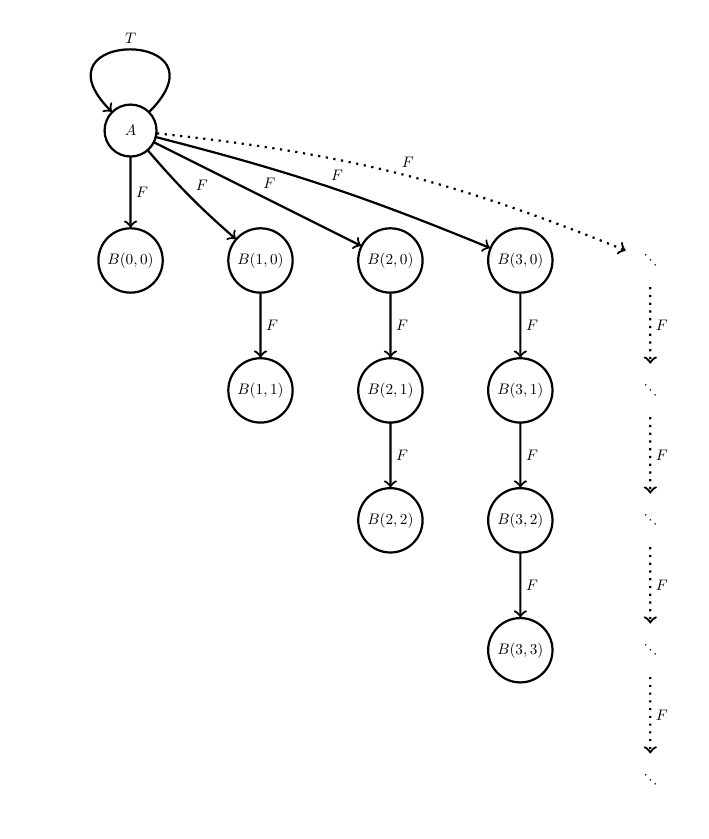
\begin{tikzpicture}[term/.style={circle,draw,minimum size=12mm,inner sep=4pt},auto , scale=0.55, every node/.style={scale=0.55}]
    \node [thick] (A) at (0,0) [term] {$A$};
    \node [thick] (B00) at (0,-3) [term] {$B(0,0)$};
      \node [thick] (B10) at (3,-3) [term] {$B(1,0)$}; \node [thick] (B20) at (6,-3) [term] {$B(2,0)$}; \node [thick] (B30) at (9,-3) [term] {$B(3,0)$}; \node[inner sep=10, rotate=-45] (B40) at (12,-3) {$\cdots$};
    \node [thick] (B11) at (3,-6) [term] {$B(1,1)$}; \node [thick] (B21) at (6,-6) [term] {$B(2,1)$}; \node [thick] (B31) at (9,-6) [term] {$B(3,1)$}; \node[inner sep=10, rotate=-45] (B41) at (12,-6) {$\cdots$};
    \node [thick] (B22) at (6,-9) [term] {$B(2,2)$}; \node [thick] (B32) at (9,-9) [term] {$B(3,2)$};
\node[inner sep=10, rotate=-45] (B42) at (12,-9) {$\cdots$};
    \node [thick] (B33) at (9,-12) [term] {$B(3,3)$};
    \node[inner sep=10, rotate=-45] (B43) at (12,-12) {$\cdots$};
    \node[inner sep=10, rotate=-45] (B44) at (12,-15) {$\cdots$};
%    
    \draw [->,thick,loop] (A) to node[above] {$T$} (A);
    \draw [->,thick] (A) to node {$F$} (B00);
    \draw [->,thick, bend right=4] (A) to node {$F$} (B10);
    \draw [->,thick] (A) to node {$F$} (B20);
    \draw [->,thick, bend left=4] (A) to node {$F$} (B30);
    \draw [->,thick, dotted, bend left=8] (A) to node {$F$} (B40);
%    
    \draw [->,thick] (B10) to node {$F$} (B11);
%
    \draw [->,thick] (B20) to node {$F$} (B21); \draw [->,thick] (B21) to node {$F$} (B22);
%   
    \draw [->,thick] (B30) to node {$F$} (B31); \draw [->,thick] (B31) to node {$F$} (B32); \draw [->,thick] (B32) to node {$F$} (B33);
%
    \draw [->,thick, dotted] (B40) to node {$F$} (B41); \draw [->,thick, dotted] (B41) to node {$F$} (B42); \draw [->,thick, dotted] (B42) to node {$F$} (B43); \draw [->,thick, dotted] (B43) to node {$F$} (B44);
  \end{tikzpicture}
\end{center}

\newcommand{\StrB}{\operatorname{Stream}(B)}
\newcommand{\NodeG}{\operatorname{Node}}

The graph $G$ is an element of a \emph{type} of graphs with nodes $A$ or $B(n,m)$ (with $m\leq n$) and with
edges labelled with a boolean $T$ or $F$. We assume that this type of graphs is available in Iris, just like we assumed that
the type of finite mathematical sequences is, see Section~\ref{sec:basic-separation-logic}. We also assume that
the type of nodes is available and denote it by $\NodeG$.
Moreover, we assume that we have an Iris type of mathematial streams (finite or infinite sequences) available; we write
$\operatorname{Stream}(B)$ for the type of streams of booleans $B=\{T,F\}$, and we write $[]$ for the empty stream,
and $l::ls$ for the stream with head $l$ and tail $ls$.

We will now consider different ways of defining reachability in the graph $G$.
Specifically, we will define predicates that express that, starting from some specific node,
a stream of booleans is reachable in $G$.
(For example, looking at the picture of $G$ above, since there is a loop from node $A$ to $A$
labelled $T$, it is intuitively clear that the constant infinite stream of $T$'s is reachable from $A$.)
Thus we will be interested in predicates on the type $\tau=\NodeG\times \StrB$.

Consider now the following function $F: (\NodeG\times \StrB\to\Prop) \to (\NodeG\times \StrB\to\Prop)$:
\begin{align*}
  F \psi = \lambda (x, ls).\,
    ls = [] \lor
    \exists y, l, ls'.\, ls = l::ls' \land \operatorname{Edge}(G,x,y,l) \land \psi y ls'
\end{align*}
where $\operatorname{Edge}(G,x,y,l)$ means that there is an edge from node $x$ to node $y$ in the graph $G$ with label $l$.

\begin{lemma}
  $F$ is monotone.
\end{lemma}

Since $F$ is monotone, the least and greatest fixed points $\lfp F$ and $\gfp F$ of $F$ exist,
as does the guarded recursive predicate $\grd F$. Each of these define a notion of reachability.


\begin{lemma}
  \label{lem:lfp-gfp-grd}
  \begin{align*}
    \forall x:\tau.\,
    \lfp F x \proves \gfp F x \proves \grd F x.
  \end{align*}
\end{lemma}

The following lemmas express that the inductive notion of reachability
only contains finite paths. 

\begin{lemma}
  \label{lem:lfp-finite}
  Let $ls$ be a \emph{finite} sequence of constant $T$'s or constant $F$'s.
  Then $\lfp F (A,ls)$ holds.
\end{lemma}

\begin{lemma}
  \label{lem:lfp-infinite}
  Let $ls$ be an \emph{infinite} sequence of constant $T$'s or constant $F$'s and let $n$ be any node.
  Then $\lfp F (n,ls)$ does not hold, (i.e., $\lfp F (n,ls) \proves \FALSE$).
\end{lemma}

The following lemmas express that the coinductive notion of reachability
not only includes finite paths, but also infinite paths.


\begin{lemma}
  Let $ls$ be the \emph{infinite} sequence of constant $T$'s.
  Then $\gfp F (A,ls)$ holds.
\end{lemma}

\begin{lemma}
  Let $ls$ be the \emph{infinite} sequence of constant $F$'s and let $n$ be any $B$ node.
  Then $\gfp F (n,ls)$ does not hold (i.e., $\gfp F (n,ls) \proves \FALSE$).
\end{lemma}

\begin{lemma}
  Let $ls$ be the \emph{infinite} sequence of constant $F$'s and let $n$ be any node.
  Then $\gfp F (n,ls)$ does not hold (i.e., $\gfp F (n,ls) \proves \FALSE$).
\end{lemma}

Intuitively, the following lemma captures that guarded-recursive predicates are ``closed under limits'':
by Lemmas \ref{lem:lfp-gfp-grd} and \ref{lem:lfp-finite} every finite path of constant $F$'s is in the guarded-recursive notion of reachability;
this is used to prove the following lemma, which says that also the limit, the \emph{infinite} sequence of constant $F$'s, is in the guarded-recursive notion of reachability.

\begin{lemma}
  Let $ls$ be the \emph{infinite} sequence of constant $F$'s.
  Then $\grd F (A,ls)$ holds.
\end{lemma}

We finally remark that guarded-recursive predicates are in fact unique (we did not include a proof rule expressing that in Section \ref{sec:recursively-defined-pred}) and that is exactly because their behaviour at limit points is determined by what happens at finite approximants.


%%% Local Variables:
%%% mode: latex
%%% TeX-master: "../main.tex"
%%% End:
